% Drawing 154/01-10 -- folder 154, batch 01, archive page 16 (PDF page 17).
% Transcription: figure : à gauche, un triangle de spécialisation $T$ hachuré entre deux pseudo-droites orange et la droite jaune ; à droite, un faisceau de droites orange au-dessus d'un arc vert, avec une petite flèche verticale. $\mathbf{N}^{*}$ rend son N ajouré suivi d'une étoile
% Kind: specialisation triangle; pencil over an arc. Method 2 (schematic redraw from the facsimile). Status: ok.
% Notes: Left: three orange pseudolines over the yellow line, the specialisation triangle T between two of them and the yellow line hatched in pencil, a fourth short orange stroke to the right. Right: a pencil of four orange lines over a dark green arc, another orange stroke to its left, and a small vertical arrow. The brown arrow-star diagrams higher on the page are not covered by this mark.
% Coordinates: 1 unit = 1 mm = 1/100 of the crop width (bbox in page fractions: [0.134, 0.412, 0.334, 0.473]).
% Redrawn by Claude (claude-opus-5-5), issue #73, 2026-11-07; not checked by a human; not compiled (no TeX in the session).
% Rights: reproduces part of the work -- behind RENDER_TRANSCRIPTS, never published by itself.
\documentclass[tikz,border=3pt]{standalone}
\usepackage{amsmath,amssymb}
\usetikzlibrary{patterns,arrows.meta}
\tikzset{Or/.style={orange!90!black}, Ye/.style={yellow!80!orange}, Lg/.style={green!60!black!70}, Dg/.style={green!45!black}, Br/.style={brown!80!black}, Rd/.style={red!85!black}, Bl/.style={blue!70!black}, Gy/.style={black!40}, pencil/.style={black!45}, struck/.style={black!35}, mark/.style={circle,draw,inner sep=1.3pt}, pt/.style={circle,fill,inner sep=0.9pt}, opt/.style={circle,draw,fill=white,inner sep=1.1pt}}
\begin{document}
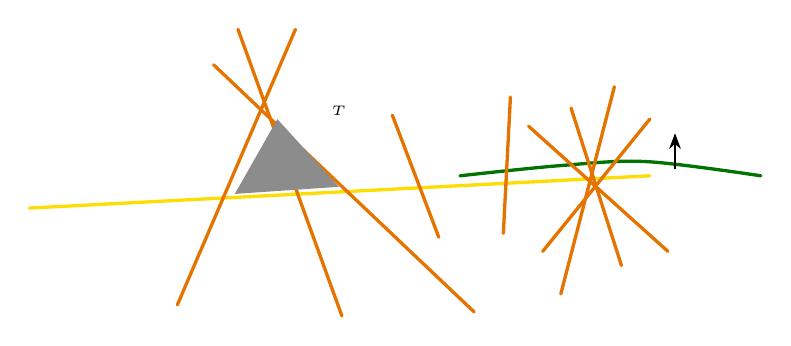
\begin{tikzpicture}[x=1mm,y=1mm,line cap=round,line join=round,font=\scriptsize]
\draw[Ye,very thick] (3,-26.8) -- (81.8,-22.7);
\draw[Or,very thick] (36.8,-4.1) -- (21.8,-39.1);
\draw[Or,very thick] (29.5,-4.1) -- (42.7,-40.5);
\draw[Or,very thick] (26.4,-8.6) -- (59.5,-40);
\draw[Or,very thick] (49.1,-15) -- (55,-30.5);
\fill[pattern=north east lines,pencil] (29.1,-25) -- (34.5,-15.5) -- (42.3,-24.1) -- cycle;
\node[inner sep=1pt] at (42.3,-14.5) {\tiny $T$};
\draw[Dg,very thick] plot[smooth, tension=0.55] coordinates {(57.7,-22.7) (70.5,-21.4) (81.4,-20.9) (95.9,-22.7)};
\draw[Or,very thick] (77.3,-11.4) -- (70.5,-37.7);
\draw[Or,very thick] (71.8,-14.1) -- (78.2,-34.1);
\draw[Or,very thick] (66.4,-16.4) -- (84.1,-32.3);
\draw[Or,very thick] (81.8,-15.5) -- (68.2,-32.3);
\draw[Or,very thick] (64.1,-12.7) -- (63.2,-30);
\draw[-{Stealth[length=2mm]}] (85,-21.8) -- (85,-17.3);
\end{tikzpicture}
\end{document}
